% author:         zhangyi zju_cs
% course:         生物智能与算法
% teacher:        yuanxi
% environment:    ubuntu 16.04
%                 texlive-full
%                 texlive-xetex
% editor:         vscode
%                 latex-workshop
% compiler:       xelatex
%                 bibtex

\documentclass[a4paper]{article}

\usepackage{ctex}           % support chinese
\usepackage{geometry}       % setting margin
\usepackage{setspace}       % setting space
\usepackage{algorithm}      % support pseudocode
\usepackage{algpseudocode}  % support pseudocode
\usepackage{caption}        % support caption
\usepackage{amsmath}        % support newtheorem
\usepackage{graphicx}       % support insert iamge

\newtheorem{definition}{\hspace{2em}定义}
\renewcommand{\algorithmicrequire}{\textbf{输入:}}


\title{多种群协同演化}
\date{2018-04-30}
\author{张毅\hspace{1em}21721190}

\geometry{left=3.5cm,right=3.5cm,top=4.5cm,bottom=4.5cm}
\setcounter{tocdepth}{3}
\doublespacing

\begin{document}
    
    %%%%%%    标题页    %%%%%%%%%%%%%%
    \pagenumbering{gobble}
    \maketitle


    %%%%%%    目录页    %%%%%%%%%%%%%%
    \newpage
    \tableofcontents
    

    %%%%%%    引言页    %%%%%%%%%%%%%%
    \newpage
    \pagenumbering{arabic}
    \section{引言}

    演化算法(Evolutionary algorithm, EA)是模拟生物遗传演化规律的一类启发式算法。由于其整体搜索策略和优化计算不依赖梯度信息,相比其他传统的局部搜索启发式算法,演化算法在搜索空间高度模态化,不连续或高度受限时具有明显优势。演化算法具有自组织、自适应、自学习的特性,能够不受问题性质的限制,有效地处理传统优化算法难以解决的复杂问题\cite{sun_ea}。但是,演化算法也存在一些限制:1)当问题的搜索空间非常大,其定义为两个或者多个互相交互的子空间的笛卡尔乘积时,演化算法很难进行有效的搜索。在极端的情况下,搜索空间可能会无限大,演化算法的搜索需要能够聚焦在相关的区域中。2)当没有内在的客观度量来评估个体适应度时演化算法很难适用。比如:不断演变的游戏策略。3)在搜索复杂结构的空间时,如果没有进行特定域的修改来帮助指导搜索,演化算法也很难适用。为解决演化算法存在的问题,协同演化算法被提出来。
    
    协同演化算法(Coevolutionary algorithm, CEA)是演化算法的扩展,相比演化算法,其个体适应度的计算是主观的,根据他们与其他个体的相交互来评估的,交互伙伴可以是同一种群的个体或者不同种群的个体\cite{wiegand2003analysis}。根据交互的性质,协同演化算法可以分为两大类:竞争型协同演化算法与合作型协同演化算法。对于合作型协同演化算法,个体如果与其他个体一起协作良好将获得奖励,协作不佳则受到惩罚。例如,在一个协同演化算法中,每个种群代表一个大问题的一个子问题,合作演化的任务就是每个种群为了解决大问题而演化出越来越适合的子问题的解。对于竞争型协同演化算法,个体获得的奖励是与他们互动的个体付出的代价。例如,捕食-被捕食模型中,其中一个种群中的个体代表某种设备(例如,排序网络),另一个种群中的个体代表该设备的输入(例如,数据),第一个种群中个体的目标是发展越来越好的设备来处理输入,而第二群人的目标是为该设备演化出越来越难的输入。


    %%%%%%    相关研究    %%%%%%%%%%%%%%
    \newpage
    \section{相关研究}
    
    1991年,Hillis等人首次对具有捕食-被捕食关系的两个对立种群(排序网络与数据集)进行协同演化\cite{hillis1990co}。其中,在第一个种群中的每个个体代表一个潜在的排序网络,其适应度的计算依赖于它对‘数据集’种群的排序效果。在另一个种群中的每个个体代表一个潜在的数据集,其适应度的计算依赖于混淆‘排序网络’种群的程度。
    
    在过去的研究中,竞争型协同演化算法在协同演化算法中占主导地位,其被广泛应用于游戏策略领域\cite{rosin1995methods,pollack1998co}。1993年,Angeline和Pollack提出竞争适应度的概念来提供比独立适应度函数更加鲁棒的训练环境,其展示了竞争对演化过程的有效性。1994年,Schlierkamp-Voosen等人成功地将竞争型协同演化应用于他们的育种遗传算法。当前,竞争型协同演化算法也已经被应用于各种机器学习问题。
    
    1994年,Potter和De Jong为研究合作型协同演化算法打开了大门\cite{potter1994cooperative},他们为这种模型开发了一个相对一般的框架,并首先应用于静态函数优化,其后又将其应用于神经网络学习。在Potter的模型中,每个种群都包含代表一个大问题中某个子问题的个体,这些种群的演化几乎是独立发生的,彼此协调,相互作用只是为了计算适应性。这样的过程可以是静态的,其子问题的划分是事先确定的且从不会改变,或者也可以是动态的,其在运行过程中可以添加或移除子问题的数量。1997年,Eriksson和Olsson使用合作协同演化算法进行库存控制优化。


    %%%%%%    协同演化    %%%%%%%%%%%%%%
    \newpage
    \section{协同演化算法}

    本章的开始,我们首先给出协同演化算法的定义。
    
    \begin{definition}
        协同演化算法:协同演化算法一种演化算法,其中个体的适应度其与其他个体相互作用的主观函数。
    \end{definition}

    协同演化的含义是几个适应度相关联的种群的同时演化,图1是两个种群协同演化的示意图,引入协同演化的实质是改进个体生存能力的评价方法:个体的适应度不仅与自己有关, 还受与之发生相互关系的其它个体的影响。根据所发生的相互关系的不同特点,协同演化算法大体可以分为如下两种:竞争型协同演化算法和合作型协同演化算法。

    \begin{figure}[H]
        \centering
        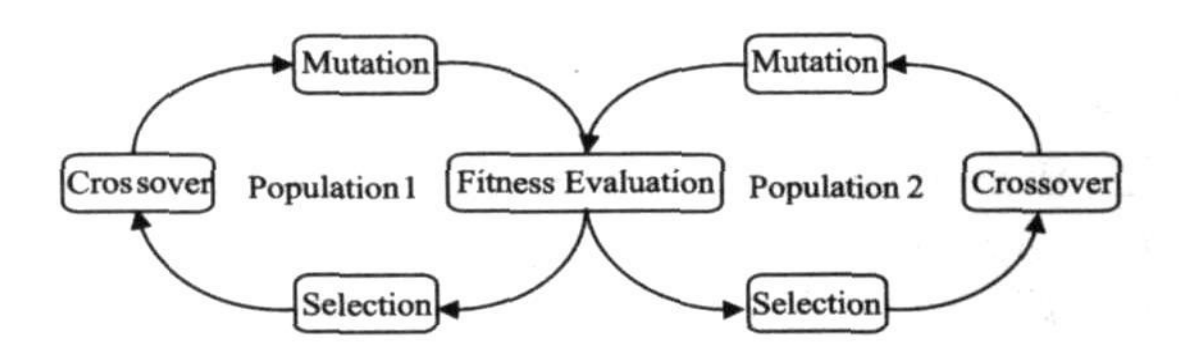
\includegraphics[width=0.8\linewidth]{./images/cea_framework.png}
        \caption{The overall framework of CEA}
        \label{fig:cea_framework}
    \end{figure}

    \subsection{竞争型协同演化算法}
    
    竞争型协同演化算法是对自然界中捕食现象的模拟:捕食者和被捕食者之间相互产生有害的影响 ,捕食者和被捕食者的任何一方的进步都会威胁另一方的生存能力。捕食者和被捕食者的生存能力都不完全由本身决定,还受到对方的影响\cite{li}。捕食者为了捕获被捕食者的生存压力会刺激捕食者的演化,被捕食者为了逃脱被捕食的生存压力也会刺激被捕食者逐渐演化。捕食者和被捕食者相互刺激对方而协同演化。

    \subsubsection{竞争型协同演化算法适应度计算}

    在竞争型协同演化算法中,个体的适应度称为做竞争适应度,竞争适应度决定于个体与竞争对手竞争中的表现。同一个体,可能由于临时竞争对手的不同,而得到不同的竞争适应度,所以竞争型协同演化算法中的竞争适应度是一种相对适应度。

    称被评估竞争适应度的个体为“学习者”,竞争对手称为“评价者”。令$L$为学习者的集合,$E$为评价者的集合。

    一种计算竞争适应度的原始方法是“简单竞争适应度”,其思想就是统计每个学习者所打败评估者的次数,可以用公式(1)表示:
    \begin{equation}
		\forall i \in L \Rightarrow CF_i = \sum_{j \in E,\;i\;defeat\;j}1
    \end{equation}
    这种竞争适应度的计算方法容易导致“转圈”等弊端。常用的竞争适应度计算方法为“共享竞争适应度”,可以用公式(2-3)表示:
    \begin{equation}
		\forall j \in E \Rightarrow N_j = \sum_{k \in L,\;k\;defeat\;j}1
    \end{equation}
    \begin{equation}
		\forall i \in L \Rightarrow CF_i = \sum_{j \in E,\;i\;defeat\;j}\frac{1}{N_j}
    \end{equation}
    “共享竞争适应度”的思想是:一个学习者能够击败的评价者越多,学习者的适应度可能越大。所以,在生存的压力下,由于评价者的激励,学习者的总体适应度水平会逐渐升高。同时,一个学习者如果能够击败一个很少有其它学习者能够击败的评价者,那么这次击败对这个学习者的适应度能够贡献一个较大的增量,因为总值为1的适应度被平均分配给较少的学习者。反之,一个能被学习者击败的评价者同时也被很多其它的学习者击败,那么这次击败对这个学习者的适应度只能够贡献一个较小的增量。

    \subsubsection{竞争型协同演化算法框架}
    竞争型协同演化算法中的个体轮流担任学习者和评价者的角色,轮流给对方施压,轮流刺激对方总体适应度水平的提高,从而以一种“军备竞赛”的方式寻找最优解。其演化过程可以用如下伪代码表示:

    \begin{algorithm}[H]
        
        \caption{the framework of Competitive Coevolutionary algorithm}
        \label{alg1}
        \onehalfspacing

        \begin{algorithmic}[1]
            \State{Begin}
            \State{Initialize $Pop_1$,$Pop2$}
            \State{Let $Pop_1$ serve as learner}
            \State{Select the set of evaluators from $Pop_2$}
            \While{not termination}
                \State{Evaluation(learner)}
                \State{Select(learner)}
                \State{Crossover(learner)}
                \State{Mutate(learner)}
                \State{Interchange the individuals in $Pop_1$ and $Pop_2$}
                \State{Select the set of evaluators from $Pop_2$}
            \EndWhile
            \State{End}
        \end{algorithmic}

    \end{algorithm}

    \subsubsection{竞争型协同演化算法应用}

    竞争型协同演化算法既能在单种群中,也能在多种群中应用。基于单种群的协同演化算法是通过同一种群内个体之间的竞争来实现的,任何一个个体都是演化中的学习者,任何一个个体都可以作为其它个体的评价者。基于单种群的协同演化算法已经成功地应用到了智能游戏,函数优化。基于多种群的协同演化算法,通过模拟生态演化中的捕食关系来实现协同演化,不同的种群轮流担任学习者和评价者的抉择,其已经成功地应用到了智能游戏、函数优化、多目标优化、最小路径分类网、模式分类、细胞自动机规则训练、非线性控制器的设计、人工神经网络等领域。

    \subsection{合作型协同演化算法}

    合作型协同演化算法是采用“分而治之”的思想,把一个问题分解成几个部分分别求解。合作型协同演化算法一般应用于可以自然地进行分解问题的情形下,合作型协同演化算法已经成功地应用到了函数优化、生产调度、人工神经网络设计,以及计算机视觉等领域。

    \subsubsection{合作型协同演化算法框架}
    合作型系统演化算法包含处于合作关系的多个种群在同时演化,种群中的每一个个体只表示解的一个部分。合作型系统演化算法的每一个子种群求一个部分解,把多个子种群的最终解按顺序连接起来就是问题的解。。其演化过程可以用如下伪代码表示:

    \begin{algorithm}[H]
        
        \caption{the framework of Cooperative Coevolutionary algorithm}
        \label{alg2}
        \onehalfspacing

        \begin{algorithmic}[1]
            \State{Begin}
            \State{Set the number of populations $N$}
            \For{$i=1;i<=N;i++$}
                \State{Initialize($Pop_i$)}
            \EndFor
            \For{$i=1;i<=N and not termination;i++$}
                \For{$j=1;j<=N and j<>i;j++$}
                    \State{ $Pop_i$ cooperate with $Pop_j$ }
                \EndFor
                \State{Select($Pop_i$)}
                \State{Crossover($Pop_i$)}
                \State{Mutate($Pop_i$)}
            \EndFor
            \State{$Solution$=NULL}
            \For{$i=1;i<=N;i++$}
                \State{$Solution$=combine($Solution$,$solution_i$)}
            \EndFor
            \State{End}
        \end{algorithmic}

    \end{algorithm}

    合作型协同演化算法引入了多个子种群,每个子群体对应一个子任务(例如多个参数中的一个)。在应用合作型协同演化算法时,首要的工作是进行任务的分解。如果任务是确定3个参数的取值,那么就可以把整个种群分为3个子群体。合作型系统演化算法的物理实现可以采用粗粒度的并行模型,每一个处理器对应一个子群体。

    \subsubsection{合作型协同演化算法适应度计算}

    传统演化算法中的个体代表一个完整的解,个体的适应度表示解的性能。在合作型协同演化算法中,子群体中的任何一个个体只是完整解的一个部分,个体的适应度表现为与其它各子群体中的个体的合作能力。为了求得某子群体中的一个个体的适应度,该子群体先把个体发送至“领域模型”,“领域模型”同时从其它的每一个子群体接收若干“合作者”来同那个个体合作,一起组成若干完整的解。领域模型把求得的适应度中的最佳值作为所求个体的适应度发送给子群体。
    
    个体适应度可以根据个体的模板来计算。具体方法是:把子群体中的个体看成完整解模板中的确定部分,而其它的部分是不确定的,该个体的适应度为模板中的部分个体的平均适应度,这种方法的实质是随机产生若干合作者。例如子种群1中个体1是“101”,其模板是“101------”。根据模板随机生成2个个体:“101000101”,“101110001”,把这两个个体的平均值作为个体“101”的适应度。
    
    合作型协同演化算法中的同一个个体,可能由于合作者的不同而得到不同的适应度值,所以其适应度也是一种相对适应度。合作型协同演化算法中的任何一个个体生存能力的体现,离不开其它的合作者。任何一个子群体的演化,对其它所有子群体都会产生正的影响。所以,合作型协同演化算法是对生态演化中互惠共生的模拟。

    \subsection{交互方法}
    
    对于协同演化算法,个体在适应度评估时,如何选择与其交互的竞争或合作者非常重要。一种最容易想到的方式是选择所有可能的合作或竞争者与其进行交互。这种方式通常成为“完全匹配”。另一个极端是个体在进行适应度评估时只与一名竞争或合作者进行交互。这种方式的一个重要问题是如何选择这个竞争或合作者。除了这两种极端的做法,还有一种就是选择竞争或合作者的某个子集与其进行交互。子集的选择可以采用随机选择或者其他方法。

    对于交互对象的选择,往往是适应度评估效果与交互计算代价的折中。对于“完全匹配”方式,每个个体的适应度计算需要与所有可能的合作或竞争者的参与,这种方式往往使适应度的计算更加可信,但是它所带来的计算代价非常大,当个体数目很大的时候,这种方式会明显增加算法的时间复杂度。而对于只选择一个竞争或合作者进行交互的方式,虽然它的计算代价非常小,但是个体适应度的计算往往与选择的交互对象直接相关,鲁棒性差。通常,折中的方式被大多数协同演化算法选择。

    %%%%%%    病态行为    %%%%%%%%%%%%%%
    \newpage
    \section{协同演化算法中的病态行为}

    \paragraph{‘梯度’消失}

    当一个种群达到某个状态时,导致其对别的种群失去相对适应性的多样性,从而使其他种群无法获得有意义的演化。竞争型协同演化中一个缺乏梯度的典型例子是:国际象棋大师扮演一个小孩进行象棋对弈。如果他没有收到比赛结果以外的任何信息,那么他几乎没有办法通过与其他小孩进行对弈来改进自己的象棋技巧。在竞争型协同演化算法中,当一个种群突然达到比其他种群更优越的水平时,就会出现‘梯度’消失,这种情况下,其无法通过竞争获得任何东西。‘梯度’消失严格意义上并不只是竞争型协同演化的问题。在更一般的情况下,包括合作型协同演化算法,‘梯度‘消失可以被看作是一个或多个种群相对于其他种群的适应度多样性的消失。也就是说:一个或多个种群突然失去多样性,导致搜索只在特定的子空间进行。

    \paragraph{相对泛化}

    当协同演化系统中的种群被吸引到空间中的某些区域时发生的行为, 其中有许多策略相对于交互伙伴的表现良好。在竞争型和合作型协同演化算法中都可以观察到这种现象。然而,对于合作型协同演化算法来说, 这个问题更加严重。这个行为反映的是协同演化系统中的自适应变化与某种绝对测度断开联系而引导结果到我们不期望的空间的行为。

    \paragraph{客观停滞}

    尽管在相互作用的个体和种群中仍有演化过程发生, 但根据某种合理的客观测度没有明显进展时发生的协同演化行为。


    %%%%%%    新的研究方向  %%%%%%%%%%%%%%
    \newpage
    \section{最新发展方向}
    
    本文在总结已有研究工作的基础上从多个角度对协同演化算法进行了介绍,本章讲对协同演化算法中出现的一些新闻题进行分析。

    \paragraph{协同演化算法的理论分析}

    关于协同演化算法与演化博弈理论之间的联系的研究目前还不成熟,它们或者是利用博弈论来进行协同演化算法的设计,或者是将协同演化算法应用于具体的工程优化问题中,并没有在优化问题空间和遗传空间建立起有效的映射。在应用这些协同演化算法时,往往缺乏对演化过程是否收敛于Nash均衡点的分析.因此,如何运用演化博弈思想对协同演化机制进行系统的分析是需要研究的问题。

    \paragraph{分布式协同演化算法}

    演化算法具有显著的隐式并行性,将分布式计算技术与协同演化算法的多种群协同演化机制结合,将建立起性能更加高效的分布式协同演化算法。

    \paragraph{协同演化算法与其他优化算法的融合}

    将协同演化思想与人工神经网络算法、人工免疫算法、模拟退火算法和蚁群算法等结合,集成现有智能算法中的不同搜索技术的一类新算法的研究已成为目前协同演化算法研究的一个热点。作为演化算法的一种新方法才刚刚兴起,在理论和实践上有许多问题需要未来进行深人的研究和探索。

    \paragraph{演化算法与多智能体系统理论的结合}
    多智能体理论和技术的研究是目前国际人工智能界研究的热点之一。因此,随着多智能体系统理论和技术的El趋完善,将多智能体系统有关竞争、协调、通信、学习、合作与协商等机制运用于协同演化的研究,可以设计一类全新的演化算法称为多智能体协同演化算法,这是协同演化算法未来值得研究的一个方向。



    %%%%%%    索引页    %%%%%%%%%%%%%%
    \newpage
    \bibliography{cea}
    \bibliographystyle{ieeetr}

\end{document}